
\section{Preliminary}
%\textcolor{red}{@Mehdi: Explain core technical concepts (needed in this paper) and related works for each area. }

\subsection{The Road to RPKI: Securing the BGP Ecosystem}
\md{The Border Gateway Protocol (BGP) has served as the basis for the Internet's routing for decades~\cite{lougheed1990rfc1163}, designed primarily for global reachability via flexible, policy-driven path selection. However, BGP’s initial design prioritized scalability and autonomy over security, assuming an implicit trust model in which route announcements are accepted without verification. This architectural gap has led to serious vulnerabilities, such as prefix hijacking~\cite{prefixHijacking} and route leaks~\cite{McDanielSS21BGPLeak}, where malicious or misconfigured ASes redirect traffic by claiming unauthorized ownership of IP resources.}

\md{Early efforts to secure BGP, such as BGPsec~\cite{rfc8205BGPSec}, aimed to provide full-path validation but failed to gain traction due to high computational overhead, significant hardware requirements, and the ``all-or-nothing'' nature of its deployment. Consequently, the networking community shifted its focus toward the Resource Public Key Infrastructure (RPKI)~\cite{RPKI}. Similar to the Web PKI used for SSL/TLS, RPKI provides a cryptographically verifiable hierarchy that roots Internet resources (IP addresses and ASNs) in a chain of trust managed by the five Regional Internet Registries (RIRs).}

\md{Under this framework, network resource owners register their prefixes by creating RPKI objects, most notably the Route Origin Authorization (ROA). An ROA is a digitally signed record that explicitly maps a specific IP prefix to its authorized origin AS for prefix announcement. Since its standardization in 2012, RPKI has become the primary mechanism for Route Origin Validation (ROV). However, as the global routing landscape evolves, the transition to RPKI becomes difficult~\cite{KangLRKC24IRRedicator, testart2020filter, nro2026rpki}. Therefore, recent research focuses on improving RPKI adoption by reducing deployment overhead~\cite{chung2019rpki, ni2025address}, mitigating operational risks~\cite{li2025improv, chen2025right}, and extending security beyond simple origin validation~\cite{hoger2025xbgpsec, rfc9234}.}

% \subsection{Border Gateway Protocol (BGP): Topology and Behavior}
% The Border Gateway Protocol (BGP) is the core inter-domain routing protocol that enables Autonomous Systems (ASes) to exchange reachability information across the Internet ~\cite{lougheed1990rfc1163}. Despite its critical role, BGP operates largely on implicit trust: route announcements are accepted without strong validation of origin or propagation paths. While extensions like BGPsec aim to provide path security, they face limited deployment. This lack of universal trust enforcement leaves BGP vulnerable to prefix hijacking, route leaks, and other malicious manipulations.

% \subsection{Resource Public Key Infrastructure (RPKI)}
% The Resource Public Key Infrastructure (RPKI) offers cryptographic validation by binding IP prefixes to authorized origin ASes, reducing certain hijacking risks~\cite{RPKI}. However, RPKI adoption remains incomplete, covering roughly 37\% of the global routing space, and focuses only on origin validation~\cite{KangLRKC24IRRedicator, testart2020filter}. Non-RPKI ASes can still advertise unverified or bogus routes, leaving a significant portion of the Internet exposed to manipulation and policy violations.

\subsection{Decentralized Trust: Blockchain Model}
\md{Blockchain is a distributed ledger technology (DLT) that maintains a shared and unchangeable record of events across a peer-to-peer network. At its core, it provides immutability, transparency, and decentralized consensus, enabling a tamper-evident, publicly auditable system without reliance on a central authority. To function without a central authority, the network follows a consensus mechanism, which defines a set of rules that ensure that all participants agree on the state of the ledger. Common types include Proof-of-Work (PoW), which relies on computational power, and Proof-of-Population (PoP), which enforces a ``one-entity, one-vote'' model through a strict identity verification process to prevent any single participant from unfairly influencing the ledger.}

\md{The decentralized and auditable properties of blockchain have motivated its use as a security layer for the Internet's routing infrastructure, BGP. Since BGP is inherently a decentralized ``network of networks'', a shared ledger naturally reflects the Internet's topology. Recent studies, including RouteChain~\cite{saad2022routechain} and ISRchain~\cite{chen2020isrchain}, demonstrate how blockchain can track routing updates and maintain a verifiable temporal history of prefix ownership. However, while these works demonstrate the potential for decentralized trust, they face significant structural and operational limitations.}

% \subsection{Public Blockchain Consensus: Proof of Population}

% Blockchain provides immutability, distributed consensus, and tamper-evident logging, properties well-suited to BGP's trust problem~\cite{zhang2019blockchain}. By enabling ASes to collaboratively record and verify routing events, blockchain ensures that misbehavior is permanently auditable and subject to consensus-based validation. Prior work, such as RouteChain~\cite{}, demonstrated how blockchain can support collective anomaly detection and route decision-making, extending security beyond RPKI's partial coverage.


\section{Motivating BGP-Sentry}\label{sec:motivation}
\textcolor{red}{@Mehdi: Add visualized evidence to justify each. }

Securing trust in the BGP protocol presents multifaceted challenges that existing solutions do not address. Although RPKI has been proposed as a potential solution, it alone is not sufficient to achieve robust BGP security. We identify three critical challenges that explain why current approaches, including RPKI and blockchain-based solutions, leave BGP vulnerable. These limitations motivate our work to design BGP-Sentry, a blockchain-based trust-expansion framework.
%This limitation is particularly alarming given that BGP vulnerabilities now threaten not only Internet availability but also financial assets in decentralized environments.
%For instance, the April 2018 MyEtherWallet attack exploited BGP by hijacking Amazon Route 53 prefixes, enabling attackers to steal over \$150,000 worth of Ether in under two hours~\cite{routingattack}, underscoring the urgent need for stronger protections. 

%The NRO RPKI Economy Adoption dataset provides daily global snapshots quantifying the percentage of advertised IPv4 and IPv6 address space per country that is cryptographically protected by Route Origin Authorizations (ROAs), serving as the authoritative metric for measuring the 'signing' phase of RPKI deployment.
\begin{figure}
    \centering
    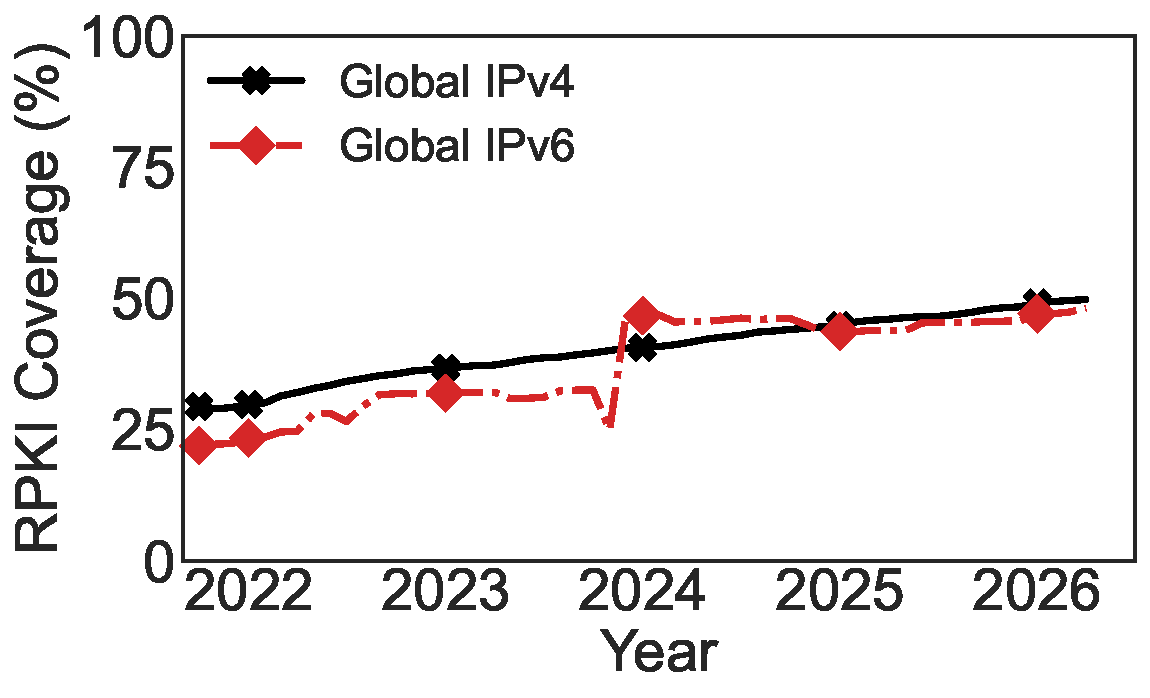
\includegraphics[width=0.35\textwidth]{Global_RPKI.pdf}
    \caption{Global RPKI adoption trends: growth of ROA-protected address space in IPv4 and IPv6 over the last 5 years.}
    \label{fig:RPKI_cov}
\end{figure}

\subsection{Structural Barriers to Universal RPKI Deployment} \md{With over 70,000 Autonomous Systems (ASes) on the Internet, only 28\%~\cite{KangLRKC24IRRedicator, testart2020filter} have adopted RPKI. Figure~\ref{fig:RPKI_cov} shows the slow RPKI coverage trend for both IPv4 and allocated IPv6 space (excluding reserved IP addresses) over the last five years, based on monthly snapshots from the NRO (Number Resource Organization)~\cite{nro2026rpki}, which tracks the global progress of ROA-protected resources. As shown, this relatively small group of ASes covers 49\% of the total IPv4 space as of April 1st, 2026.  Additionally, a recent study~\cite{qin2024understanding} demonstrated that even among ASes that have adopted RPKI, 61.3\% still accept and propagate invalid RPKI announcements received from their customers, which highlights a strong disconnect between RPKI registration and the real-world enforcement, where the operational costs and risks of strict filtering often outweigh the immediate benefits for network operators.}

\md{This limited adoption since the standardization in 2012 suggests that RPKI is unlikely to ever achieve universal coverage, particularly as operational priorities continue to overrule security incentives in the face of systemic barriers such as technical complexity, deployment costs, policy fragmentation, and geopolitical constraints. Although recent research has focused on strengthening the RPKI itself~\cite{hoger2025xbgpsec, ni2025address, li2025improv, chen2025right}, these efforts do not address the core issue of partial adoption. A substantial fraction of ASes will likely remain outside the RPKI ecosystem due to resource limitations or organizational resistance. However, these networks are integral to the Internet's operation, and their insecurity can have global repercussions. Therefore, rather than assuming full RPKI adoption, this work proposes a practical BGP security solution that accounts for this heterogeneity and develops mechanisms to extend trust and validation beyond the RPKI-enabled portion of the Internet.}


% The RPKI deployment covers only about 37\% of Autonomous Systems~\cite{KangLRKC24IRRedicator, testart2020filter}, leaving a significant portion of the Internet without cryptographic validation. This incomplete coverage stems from economic incentive misalignment, where RPKI-adopting ASes bear deployment and maintenance costs while providing security benefits to the entire ecosystem without recognition or rewards, creating a classic chicken-and-egg problem where ROA creation is only valuable if networks perform validation, while validation deployment is only worthwhile if sufficient ROAs exist. Non-RPKI ASes can "free-ride" on security improvements provided by RPKI adopters without contributing to the system or being held accountable, while detection and threat mitigation efforts by RPKI participants protect non-participants without compensation or responsibility sharing.

% RPKI will never achieve 100\% coverage due to various systemic barriers, including technical complexity, financial constraints, policy disagreements, and political considerations that prevent universal adoption. In the research community, the trend is more on enhancing the RPKI technology, like keeping records in the blockchain \cite{saad2022routechain}. Even if we make RPKI more robust and efficient, a substantial portion of ASes will remain outside the RPKI ecosystem due to deployment challenges, resource limitations, or organizational resistance. We cannot simply ignore or abandon these non-RPKI ASes, as they represent critical parts of the Internet infrastructure, and their vulnerabilities affect the entire routing ecosystem. Thus, any comprehensive BGP security solution must find ways to extend trust and validation to the non-RPKI portion of the Internet rather than writing them off as perpetually insecure.


\begin{figure}[t]
\centering
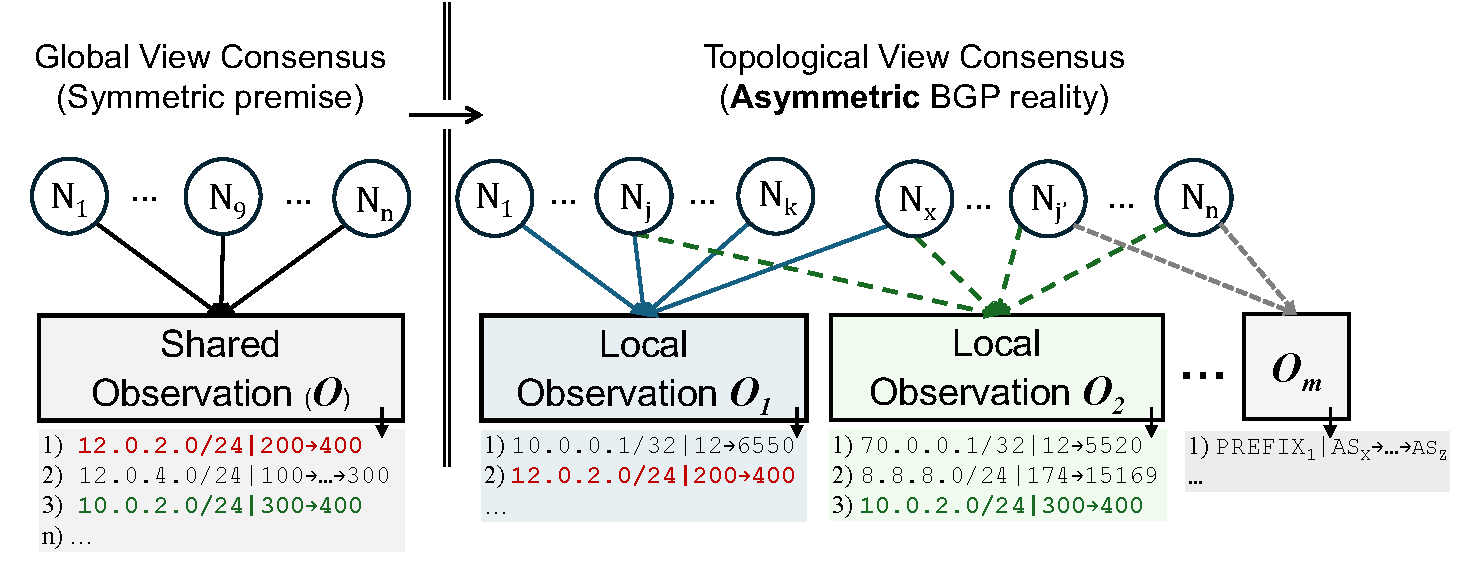
\includegraphics[width=0.48\textwidth]{figures/BGP-Asym.pdf}
\caption{Asymmetric knowledge in BGP: In a conventional blockchain, all nodes receive a uniform global observation $O$, whereas in BGP environment, consensus inputs are heterogeneous local observations $O_i$, with each node seeing a partial view of routing events. }
\label{fig:asymmetric_knowledge}
\end{figure}

\subsection{Asymmetric Consensus in Blockchain for BGP security} 
\md{Current BGP security mechanisms, including RPKI, are fundamentally stateless. They validate routing updates in isolation, considering only transient network events and ignoring historical attack patterns or cumulative behavioral trends. While blockchain technology offers the immutability required for long-term auditing, there is currently no solution that leverages this capability to establish behavioral reputation. Without a verifiable audit trail of past incidents, it is impossible to reliably distinguish transient network anomalies from coordinated attacks such as repeated misconfigurations or systematic prefix hijacking~\cite{testart2019profiling}.}

\md{The primary barrier to establishing this historical record is the asymmetric knowledge inherent in BGP, demonstrated in Figure~\ref{fig:asymmetric_knowledge}. As shown, unlike traditional blockchains, where all nodes observe a shared transaction pool, BGP observers possess unique, vantage-point-dependent views: an observer at one router may see an announcement that is invisible or different from another. Existing blockchain-based BGP solutions lack consensus algorithms designed for this asymmetric environment. They struggle to reconcile these conflicting yet valid perspectives into a single, unified behavioral assessment. Thus, we propose a scalable consensus framework required for distributed observers to agree on an AS's historical behavior across diverse vantage points.}




% \begin{figure}[t]
% \centering
% \resizebox{\columnwidth}{!}{%
% \begin{tikzpicture}
% \begin{axis}[
%     width=7.5cm,
%     height=5.0cm,
%     xlabel={Time Since First Observer (seconds)},
%     ylabel={RPKI Validators That Received (\%)},
%     xmin=0, xmax=65,
%     ymin=0, ymax=105,
%     ytick={0,20,40,60,80,100},
%     tick label style={font=\scriptsize},
%     label style={font=\scriptsize},
%     ymajorgrids=true,
%     grid style={line width=0.2pt, draw=black!12},
%     every axis plot/.append style={line width=1.2pt},
% ]

% % Legitimate propagation curve
% \addplot[black, solid] coordinates {
%     (0,5) (2,30) (5,65.4) (8,73) (10,77.1) (15,85) (20,91) (30,97.3) (45,99.1) (60,99.2)
% };

% % Topological ceiling
% \draw[black!30, thin, densely dashed] (axis cs:0,99.2) -- (axis cs:65,99.2);
% \node[font=\tiny, text=black!40, anchor=south east] at (axis cs:64,99.2) {topological ceiling: 99.2\%};

% % Shade the temporal gap region
% \addplot[fill=black!8, draw=none, forget plot] coordinates {
%     (0,5) (2,30) (5,65.4) (8,73) (10,77.1) (15,85) (20,91) (30,97.3) (45,99.1) (60,99.2)
%     (60,99.2) (0,99.2)
% } \closedcycle;

% % Annotations
% \node[font=\scriptsize, anchor=center] at (axis cs:15,92) {temporal gap};
% \draw[-{Stealth[length=2pt]}, thin, black!60] (axis cs:15,90) -- (axis cs:10,82);
% \node[font=\scriptsize, anchor=center] at (axis cs:35,50) {received};

% % Key data points
% \node[font=\tiny, fill=white, inner sep=1pt] at (axis cs:5,60) {65\%};
% \node[font=\tiny, fill=white, inner sep=1pt] at (axis cs:10,72) {77\%};
% \node[font=\tiny, fill=white, inner sep=1pt] at (axis cs:30,93) {97\%};

% \end{axis}
% \end{tikzpicture}%
% }
% \caption{Propagation of legitimate BGP announcements to RPKI validators over time (400-AS CAIDA topology, 254~validators, mean over 1,808 prefix-origin pairs). The shaded area represents the temporal gap---validators that will eventually receive the announcement but have not yet at the given time. At 5\,s, only 65\% of validators have the information; by 30\,s, 97\% have received it. The gap between the curve and the ceiling is the consensus challenge: any voting window shorter than propagation time will exclude informed validators.}
% \label{fig:asymmetry_cdf}
% \end{figure}



%\subsection{Lacking Data Plane-aware Blockchain Consensus.} 
% Current BGP security approaches, including RPKI, operate without the ability to accumulate and maintain comprehensive security intelligence over time. Each security decision is made in isolation without considering historical attack patterns, behavioral trends, or cumulative evidence of malicious activity. This intelligence gap prevents security systems from building a comprehensive understanding of threat landscapes and distinguishing between isolated incidents and coordinated attack campaigns.


\subsection{RPKI-Blindness in Blockchain Trust Establishment} 
\md{While blockchain offers a significant opportunity to extend decentralized trust, existing blockchain-based BGP security solutions are RPKI-agnostic, particularly during the critical selection and onboarding of nodes for consensus and validation. Prior work, RouteChain~\cite{saad2022routechain}, treats all nodes as equally trustworthy despite varying levels of routing competence and security commitment. They establish trust by randomly selecting nodes regardless of their RPKI status or routing credibility, creating a circular problem in which the system relies on unverified entities to validate routing information, potentially allowing malicious or misconfigured nodes to participate in consensus decisions that affect the integrity of the global routing security. 
This motivates a mechanism that is verifiable at onboarding and incentivized to behave honestly, enabling comprehensive surveillance of the entire BGP ecosystem.}

%By failing to leverage the established cryptographic foundation of RPKI infrastructure when establishing trust, these frameworks treat all nodes as equally trustworthy despite varying levels of routing competence and security commitment. These systems allow potentially unreliable nodes to join the trusted network, compromising the integrity of the entire validation framework. 

%Without requiring demonstrated routing competence or cryptographic validation capabilities (such as RPKI deployment and ROA maintenance), blockchain-based BGP systems allow potentially unreliable nodes to join the trusted network, compromising the integrity of the entire validation framework. Therefore, an authenticated observer network, verifiable during onboarding and incentivized to operate honestly, is needed to monitor and rate the behavior of non-RPKI ASes, enabling comprehensive coverage of the entire BGP ecosystem.


Through this multi-faceted approach, BGP-Sentry enhances routing security by complementing and strengthening the current RPKI ecosystem without requiring replacement or overhaul of existing infrastructure, allowing easy adoption across the Internet routing landscape.




% The absence of persistent security intelligence severely limits the ability to perform proactive threat detection and establish context-aware security policies. Recent research highlights that many BGP incidents stem from repeated misconfigurations and systematic abuse patterns rather than isolated events~\cite{testart2019profiling}, yet current systems cannot leverage this historical context for improved security decisions~\cite{haeberlen2009netreview}.While distributed ledger technology offers immutability for tracking behavioral history, achieving consensus among BGP observers presents unique challenges. Unlike traditional blockchain systems where all nodes observe a shared transaction mempool, BGP monitoring produces fundamentally asymmetric knowledge where each observer sees only announcements reaching its edge router, and ASes can announce different routes to different neighbors based on network configurations and policies. This means distributed observers may hold conflicting yet valid views of the same routing events. Existing solutions lack consensus algorithms designed for BGP's asymmetric, high-volume environment that can scale to Internet-wide deployment while enabling observers to reliably agree on behavioral assessments despite their differing vantage points.

% \subsection{A Blockchain-based Trust Expansion Framework}
% To overcome the aforementioned challenges and provide a secure networking routing environment, we propose BGP-Sentry, a complementary blockchain-based framework that works alongside existing RPKI infrastructure and extends its capabilities. BGP-Sentry specifically addresses persistent origin validation gaps that affect all network participants, including those outside the RPKI-enabled ASes. Using RPKI-enabled ASes as a decentralized network of verified observers, BGP-Sentry enables scalable and continuous behavioral monitoring of routing announcements. It employs smart contract-based trust mechanisms on the blockchain to ensure transparency, accountability, and tamper-resistant validation, while implementing BGP Coin incentives to maintain observer honesty and participation quality.


%BGP-Sentry functions as a unified trust-expansion ecosystem that leverages the current 37\% RPKI deployment to secure the broader Internet. By onboarding RPKI-enabled ASes as \textbf{trusted observers} through a Sybil-resistant \textbf{Proof of Population (PoP)} consensus mechanism, the system establishes a decentralized monitoring layer where each verified node maintains an equal vote. These observers are economically motivated via \textbf{BGP Coin rewards} to monitor the real-time behavior of non-RPKI networks, subsequently translating these observations into immutable reputation scores on a blockchain. This integration effectively bridges the cryptographic coverage gap, transforming isolated routing events into \textbf{persistent security intelligence} that enables accountable, context-aware routing decisions across the global landscape.
%Specifically, BGP-Sentry addresses the three challenges as follows: (1) \textit{Extended Coverage and Trust Propagation:} BGP-Sentry extends cryptographic trust to networks that do not currently participate in RPKI by introducing a behavioral scoring system that evaluates the legitimacy of route announcements from non-RPKI ASes, effectively bridging the coverage gap and enabling trust propagation beyond the current 37\% RPKI deployment while implementing BGP Coin rewards for RPKI adopters and reputation-based accountability measures for non-RPKI ASes; (2) \textit{RPKI-Verified Observers with Honesty Incentives:} BGP-Sentry implements a verified onboarding process that leverages RPKI-enabled ASes as trusted observers based on their demonstrated cryptographic validation capabilities and ROA maintenance, ensuring that only verified, competent nodes participate in the blockchain consensus mechanism. BGP Coin incentives motivate active participation; observers earn coins for collecting signatures, proposing transactions to the blockchain, voting in consensus, and detecting attacks. This dual mechanism, verified identity through RPKI onboarding and sustained engagement through economic rewards, establishes a reliable observer network for monitoring non-RPKI ASes. (3) \textit{Scalable Consensus with Persistent  Intelligence:} BGP-Sentry employs a Proof of Population (PoP) consensus mechanism that ensures democratic participation, one verified node, one vote, while preventing Sybil attacks through mandatory RPKI verification during onboarding. This lightweight consensus scales efficiently to Internet-wide deployment without energy-intensive mining or stake-based plutocracy. Through blockchain's immutable ledger, the system maintains persistent security intelligence, tracking historical attack patterns, distinguishing isolated incidents from coordinated campaigns, and enabling context-aware security decisions based on cumulative threat intelligence.